\documentclass{frontiersSCNS} % for Science articles



\usepackage{graphicx}
\graphicspath{{figs/}}
\usepackage{tikz}
\usetikzlibrary{shapes}
\usetikzlibrary{svg.path}
%
\usepackage{amsmath} 
\usepackage{mathptmx}      % use Times fonts if available on your TeX system
%
\usepackage{color, soul}
\usepackage{url}
\usepackage{multirow}
\usepackage{array}
\usepackage{fixltx2e}
\usepackage{textcomp}
\usepackage{booktabs}

\usepackage{caption}
\usepackage{subcaption}
\usepackage{float}
\floatstyle{plaintop}

\usepackage{paralist} % inparaenum

\usepackage[bookmarks]{hyperref}

\usepackage[draft, nomargin, marginclue, footnote]{fixme}
\fxsetup{targetlayout=color}

\usepackage{xspace}
\newcommand{\eg}{\textit{e.g.}\xspace}
\newcommand{\etal}{\textit{et al.}\xspace}
\newcommand{\ie}{\textit{i.e.}\xspace}
\newcommand{\etc}{\textit{etc.}\xspace}
\newcommand{\vs}{\textit{vs.}\xspace}

\usepackage{xifthen}% provides \isempty test

% use either \Ant or \Ant[R,H,C,...]
\newcommand{\Ant}[1][]{%
      \ifthenelse{\isempty{#1}}%
        {$\mathcal{A}$}
        {$\mathcal{A}(#1)$}
}

\newcommand{\AntE}[1][]{%
      \ifthenelse{\isempty{#1}}%
      {$\widetilde{\mathcal{A}}$}
      {$\widetilde{\mathcal{A}}(#1)$}
}


% for use inside a math environment
\newcommand{\ant}[1][]{%
      \ifthenelse{\isempty{#1}}%
      {\mathcal{A}}
      {\mathcal{A}(#1)}
}

\newcommand{\antE}[1][]{%
      \ifthenelse{\isempty{#1}}%
      {\widetilde{\mathcal{A}}}
          {\widetilde{\mathcal{A}}(#1)}
}

\newcommand{\antENorm}[1][]{%
      \ifthenelse{\isempty{#1}}%
      {\widehat{\mathcal{A}}}
      {\widehat{\mathcal{A}}(#1)}
}

\newcommand{\IPA}{{$\mathcal{A}_0$~}}
\newcommand{\IPAe}{{$\widetilde{\mathcal{A}_0}$~}}
\newcommand{\SLA}{{$\mathcal{A}_\infty$~}}
\newcommand{\SLAe}{{$\widetilde{\mathcal{A}_\infty}$~}}
\newcommand{\sla}{{\mathcal{A}_\infty}}
\newcommand{\AntMax}{{$\mathcal{A}_{max}$~}}
\newcommand{\AntEMax}{{$\widetilde{\mathcal{A}_{max}}$~}}
\newcommand{\antEMax}{{\widetilde{\mathcal{A}_{max}}}}

\hyphenation{com-mon-ly}
\hyphenation{an-thro-po-mor-phism}
\hyphenation{an-thro-po-mor-phic}

\copyrightyear{}
\pubyear{}

\def\journal{Cognitive Science}
\def\DOI{}
\def\articleType{Research Article}
\def\keyFont{\fontsize{8}{11}\helveticabold }
\def\firstAuthorLast{Fink {et~al.}} 
\def\Authors{Julia Fink\,$^{1*\dagger}$, S\'{e}verin Lemaignan$^{1\dagger}$, Claire Braboszcz$^{2}$ and Pierre Dillenbourg$^{1}$}
\def\Address{$^{1}$Computer-Human Interaction in Learning and Instruction
    (CHILI) \\ \'{E}cole Polytechnique F\'{e}d\'{e}rale de Lausanne (EPFL) \\ CH-1015 Lausanne, Switzerland \\
\vspace{0.25cm}
$^{2}$Laboratory for Neurology and Imaging of Cognition (LabNIC) \\
Universit\'{e} de Gen\`{e}ve \\ CH-1211 Gen\`{e}ve, Switzerland 

\vspace{0.5em}\tiny{$\dagger$ These authors have equally contributed to this article.}
}
\def\corrAuthor{Julia Fink \vspace{1mm}}
\def\corrAddress{EPFL - CHILI, RLC D1 740, Station 20, CH-1015 Lausanne, Switzerland}
\def\corrEmail{julia.fink@epfl.ch}


\begin{document}
\onecolumn
\firstpage{1}

\title[Dynamics of Anthropomorphism]{Anthropomorphism in Human-Robot
Interaction: Nature, Dynamics and Underlying Cognitive Mechanisms}
\author[\firstAuthorLast ]{\Authors}
\address{}
\correspondance{}
\extraAuth{}
\topic{The Uncanny Valley Hypothesis and Beyond}

\maketitle


\begin{abstract}

\textit{Anthropomorphism} -- people's tendency to perceive human-like
characteristics in non-human agents -- is a phenomenon that is often
studied from the sole perspective of the human-like \emph{design} of robots.

By building upon experimental results from several studies, a comprehensive
synthesis of literature, as well as insights from social psychology, cognitive
science, and neuroscience, this article proposes to extend our current
understanding of anthropomorphism. We examine the several \textbf{factors} that
determine anthropomorphism, namely the design of the non-human agent, the
individual psychological determinants of the human user, and the context of use.
Moreover, we discuss several episodes of interaction that influence the
anthropomorphic projections on the robot, like the \textbf{novelty effect}, the
role of \textbf{familiarization} and the impact of \textbf{unexpected
behaviors}.

We then propose a \textbf{qualitative model} that defines a clear terminology
and accounts for the \textbf{non-monotonic dynamics} of the phenomenon. We
further relate the observed effects of anthropomorphism to their
\textbf{underlying cognitive precursors}.

Finally, the article also discusses techniques to measure anthropomorphism,
and we conclude with a few suggestions on how others can apply our model to
better describe people's tendency to perceive human-like characteristics in non-human
agents.


\tiny
 \keyFont{ \section{Keywords:} Anthropomorphism, Design, Human-Robot Interaction, Social Issues in Robotics, Acceptance of Robots}

\end{abstract}

%%%%%%%%%%%%%%%%%%%%%%%%%%%%%%%%%%%%%%%%%%%%%%%%%%%%%%%%%%%%%%%%%%%%%%%%%
%
%
%
%		INTRODUCTION & OVERVIEW
%
%
%
%%%%%%%%%%%%%%%%%%%%%%%%%%%%%%%%%%%%%%%%%%%%%%%%%%%%%%%%%%%%%%%%%%%%%%%%%


\section{Introduction}
\label{sec:intro}

The Uncanny Valley hypothesis \citep{mori_uncanny_1970} proposes that human-like
designs of objects and non-human agents can evoke both positive and negative
feelings in the human observer / user. A positive valence reflects the
experience of emotional engagement with and feelings of empathy for the
non-human agent \citep{cheetham_human_2011}. This in turn may lead to an
effective (human-like and human-social) interaction with the non-human agent,
and increase people's acceptance of it. 

A phenomenon that is often studied related to this is \textbf{anthropomorphism}.
This article aims at fostering a better understanding of anthropomorphism (noted
\Ant in this paper) in human-robot interaction by considering the phenomenon as
a whole. Robotics researchers often tend to consider that anthropomorphism only
describes a static set of human-like features of a robot (like its shape, its
speech capabilities, facial expressions, etc.). We refer to these
characteristics as the \emph{anthropomorphic design} of the
robot~\citep{fink_anthropomorphism_2012}, and propose that
\emph{anthropomorphism} in general refers to a \emph{social phenomenon} that
emerges from the (real or imagined) interaction between a non-human agent (a
robot in our case) and a human~\citep{persson_anthropomorphism_2000}.  According
to~\cite{epley_when_2008}, anthropomorphism includes the human perception of
emotional states, motivations, intentions in the non-human agent, and tends to
ascribe those qualities to it.  As such, the dynamic and socio-cognitive
dimensions of anthropomorphism are essential to understand the complex bonds
that human users build with artificial agents such as robots. This article aims
at advancing our understanding of this phenomenon, both in term of an
interdisciplinary literature synthesis, and in term of qualitative yet formal
models that will support further research in this field.

\subsection{A few results from the field}
\label{sec:field-results}

\begin{figure}[b]
        \centering
        \begin{subfigure}[t]{0.48\columnwidth}
                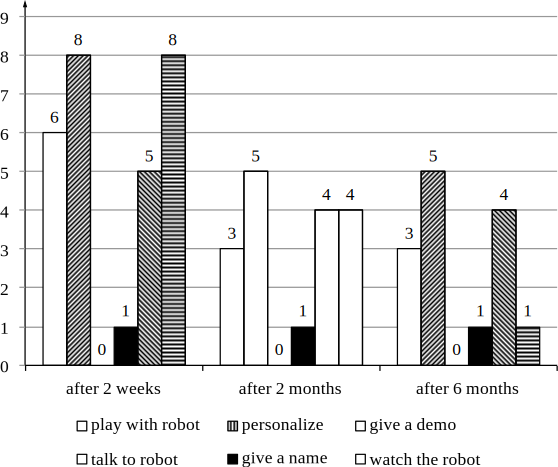
\includegraphics[height=7cm]{roomba-activities}
                \caption{Activities related to Roomba, \textit{n = 9 households}}
                \label{fig:roomba-activities}
        \end{subfigure}%
        \hspace{0.5cm} 
        \begin{subfigure}[t]{0.48\columnwidth}
                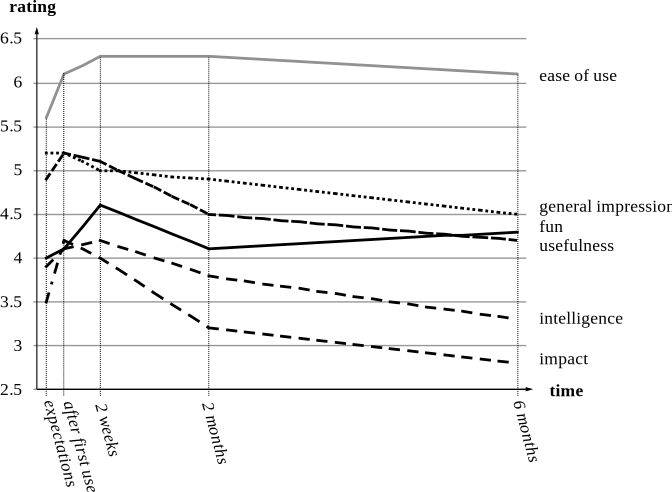
\includegraphics[height=7cm]{roomba-ratings}
                \caption{People's perception of Roomba, \textit{n = 15
                participants}}
                \label{fig:roomba-perception}
        \end{subfigure}
    \caption{Usage and perception of the Roomba vacuum-cleaning robot over a 6
    months period. Qualitative data suggest that people's activities related to
    the robot as well as their perception of the robot change over time.}
    \label{fig:roomba}
\end{figure}

To support the reflection on variances and dimensions of anthropomorphism, it is 
useful to consider a few experimental
results. We studied anthropomorphism in several short- and long-term
human-robot interaction studies that we carried out with embodied robots, both
in ecologically valid real-world environments and controlled lab settings. Those
experiments are presented in details in previously published
articles~\citep{fink_anthropomorphic_2012, fink_living_2013, fink2014which,
lemaignan2014dynamics}. We only highlight here a few qualitative results that
underline the complexity of the phenomenon.

Figures~\ref{fig:roomba-activities} and~\ref{fig:roomba-perception} give a first
perspective on how naive users interact and perceive robots over a long period
of time. \emph{Roomba} vacuum cleaning robots were given to nine
households for a 6-months period. The aim was to explore how people use and
perceive the robot over time, and how they generally live with the Roomba in
their home. At various time points, users were asked to rate their perception of
different features of the robot on a 7-point rating scale. As
Figure~\ref{fig:roomba-perception} shows, some features remained stable over
time (\emph{ease of use} and \emph{fun}), and others decreased: the perceived
\emph{usefulness}, \emph{intelligence} and \emph{impact} on their household.
\emph{intelligence} and \emph{impact} reflect the cognitive engagement of the
user towards the machine: we can assume that one does not care to engage in a
(cognitive) interaction with an artifact perceived as non-intelligent and with
no impact on one's life (and the level of activity pictured in
Figure~\ref{fig:roomba-activities} qualitatively confirms this intuition). Even
if one can argue that the Roomba is not designed to foster interaction, it
raises a first question: how to sustain engagement between a robot and a human
over a long period of time? And, as a pre-requisite to answer, do we actually
understand the psychological phenomenon, and can we effectively account for the
dynamics of these interactions?

Those questions are certainly not new, but paradoxically, while anthropomorphism
is a commonly discussed trait of human-robot interaction, it appears
that we lack formal grounds and models that would account for the long-term
dynamics of these interactions.

\begin{figure}[b]
        \centering
        \begin{subfigure}[b]{0.48\columnwidth}
                \centering
                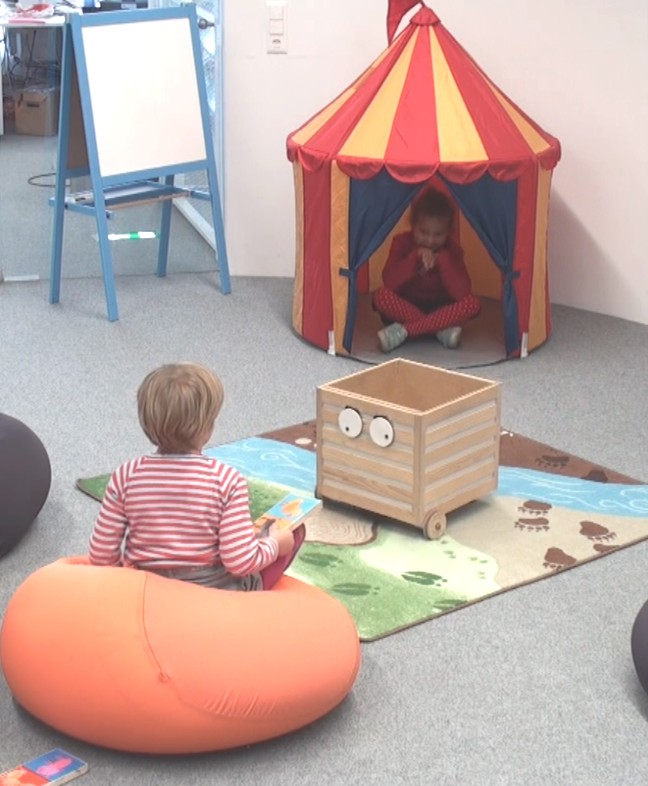
\includegraphics[width=0.75\textwidth]{ranger}
                \caption{Interaction scenario of the domino study:
                    the robot toy box \emph{Ranger} transports domino tiles between the two
                children}
                \label{fig:ranger-expe}
        \end{subfigure}%
        \hspace{0.5cm}
        \begin{subfigure}[b]{0.48\columnwidth}
            
\includegraphics[width=\textwidth]{correlation}
            \caption{\emph{Actions reflecting engagement} vs \textit{subjective anthropomorphic
                perception} evidence one cluster of
                high-anthropomorphizers/low-interactors and another group of children who
                interact more with the robot and anthropomorphize it less.}
            \label{fig:qualitative-score}
        \end{subfigure}
        \caption{Investigating children's interactions with a robot in a playful
            context: anthropomorphic perception does not necessarily positively
            correlate with engagement.}
    \label{fig:ranger}
\end{figure}


Figure~\ref{fig:qualitative-score} calls for other initial remarks. This diagram
shows data from a (yet unpublished) study in which 13 pairs of children (4-5
years old) played for about 20 minutes a domino game with a robot toy box. The
robot was tasked to carry domino pieces from one child to the other
(Figure~\ref{fig:ranger-expe}).  The $x$-axis represents the number of social
interactions between the children and the robot (like talking to the robot or
showing objects), based on video annotations. On the $y$-axis, we have a
synthetic qualitative measurement of anthropomorphic perception of the the
robot, based on two interviews with the children. The scatter plot evidences one
cluster of high-anthropomorphizers/low-interactors and a another group of
children who interact more with the robot and anthropomorphize it less: the more
the children anthropomophized, the less engaged into the interaction they were.

These results may seem counter-intuitive at first sight, and illustrate that the
mechanisms that relate anthropomorphism to adoption and engagement are
non-trivial. In section~\ref{sec:cognition-neuroscience}, we will sketch a model of
the cognitive correlates of anthropomorphism that partially account for these
results.


\subsection{Towards a formal understanding of anthropomorphism}

These first remarks lead to the main question we attempt to address in this
article: how can we understand \emph{anthropomorphism} as a whole, and in such a
way that it supports or improves the design of sustainable human-robot interaction?

We propose to discuss anthropomorphism from three complementary perspectives: 

First, by reviewing what anthropomorphism actually means: besides an
\emph{artifact-centric} understanding that explains anthropomorphism from the
human-like design of the non-human artifact, it seems important to explicit the
social component, namely a \emph{human-centric} understanding, of
anthropomorphism.

Second, we propose a qualitative model of the \textit{dynamics of
anthropomorphism} to understand how anthropomorphism evolves over time. These
dynamics are typically non-monotonic, and effects like the \emph{novelty effect} play here
a key role.

Finally, we synthetize and integrate in an explanatory model the \emph{cognitive
mechanisms} that underlie anthropomorphism. Several studies previously showed
that we build instinctive bonds with robots as soon as we attribute animacy, and
we also know from social psychology some of the mechanisms that lead to
\emph{familiarization}. We attempt here to build a practical model of the
cognitive layers we encounter in human-robot interaction.


\paragraph{Terminology used in this article\\}

Despite the fact that there is no commonly accepted definition, the terms
\textit{anthropomorphism}, \textit{anthropomorphic} or \textit{human-like} are
often used as if their meanings were clear and agreed
upon~\citep{persson_anthropomorphism_2000}. It is however argued that these
terms might be misused~\citep{duffy_anthropomorphism_2002,epley_when_2008}, and
while some researchers would refer for instance to \textit{``the robot's level
of anthropomorphism''} \citep{bartneck_is_2007,feil-seifer_human-robot_2008},
others disagree and argue that a system or artifact itself does not
\emph{contain anthropomorphism} (anthropomorphism is not intrinsic to the robot)
but only \emph{gives rise} to the process of anthropomorphizing in a given user
and situation.

In the frame of this article, we refer to the term \textbf{anthropomorphism} to
describe the \emph{psychological} phenomenon which arises in the \emph{social
context} of an interaction between a human agent and a non-human agent, in our
case a robot. We use this term to refer to both people's tendency to
\textit{perceive} (\textbf{anthropomorphic perceptions}) human-like
characteristics, and to the tendency to \textit{ascribe} or \textit{attribute}
such human-like characteristics to the agent or artifact
(\textbf{anthropomorphic projections}). Besides, we call {\bf anthropomorphic
effects} the \emph{observable manifestations} of anthropomorphism, \ie the
human's behaviors and actions toward a non-human agent that reflect the
underlying cognitive process of anthropomorphizing.

Despite the fact that ``anthropomorphism'' literally means ``human form'' we
propose that the term should \textit{not} be used to refer to the \emph{form}
and/or \emph{design} of a non-human agent or artifact. To refer to an imitation
by an artificial agent of an human-like form, we propose to use the term
\textbf{anthropomorphic design}. This explicit terminology prevents the commonly
encountered confusion between anthropomorphism as a psychological, subjective
phenomenon, and the external, objective factors that \emph{influence} the
phenomenon itself.

In the following, we might use the terms \emph{form} and \emph{design}
interchangeably. Note that the terms \textit{form} or {\it design} do not only
refer to the shape (how it looks like) but to the total expression of the
artifact~\citep{bartneck_shaping_2004}. \citet{disalvo_hug:_2003} argues that
\textit{form} includes the physical shape, materials, and behavioral qualities
of the product. The behavioral aspect is of special importance for interactive
systems that show some degree of autonomy (independence).

\subsection{Article overview}

The remainder of this article is organized as follow.  According to the three
perspectives that we take, section \ref{sec:anthropomorphism} establishes a
common ground in the understanding of anthropomorphism. We review literature
from several relevant domains and integrate the different explanations into an
understanding of anthropomorphism as a multi-factor phenomenon.  Based on this,
section~\ref{sec:our-ideas} proposes a new qualitative model of the dynamics of
anthropomorphism. This model describes the variances and dynamics of people's
tendency to anthropomorphize an artificial agent, such as a robot. Section
\ref{sec:cognition-neuroscience} then investigates the cognitive and
neuro-biological mechanisms of anthropomorphism to consolidate our
considerations and the proposed model.  Section \ref{sec:measuring} looks at how
these models can be operationalized, and in particular, what are the tools at
hand to measure anthropomorphism. Finally, section \ref{sec:conclusion}
concludes this article and offers starting points for further research on
anthropomorphism and the effect of the human-like design approach in robotics.


%%%%%%%%%%%%%%%%%%%%%%%%%%%%%%%%%%%%%%%%%%%%%%%%%%%%%%%%%%%%%%%%%%%%%%%%%
%
%
%
%		WHAT IS ANTHROPOMORPHISM
%
%
%
%%%%%%%%%%%%%%%%%%%%%%%%%%%%%%%%%%%%%%%%%%%%%%%%%%%%%%%%%%%%%%%%%%%%%%%%%

\section{The Dimensions of Anthropomorphism}
\label{sec:anthropomorphism}

Anthropomorphism arises in an interaction between a human and a non-human agent,
and one can consequently take two main perspectives when trying to explain why
humans anthropomorphize~\citep{lee_human_2005}: an artifact-centric perspective
and a human-centric perspective. We present these two perspectives, with a
special focus on the complex human aspects: we attempt there to summarize the
main approaches from developmental psychology, cognitive science, neuroscience,
and social psychology. We then briefly discuss the impact of the interaction
context on anthropomorphism, which will finally lead us to globally restate
anthropomorphism as a \emph{multi-factor phenomenon}.

%%%%%%%%%%%%%%%%%%%%%%%%%%%%%%%%%%%%%%%%%%%%%%%%%%%%%%%%%%%%%%%%%%%%%%%%%
%
%
%
%		WHY DO HUMAN ANTHROPOMORPHIZE
%
%
%
%%%%%%%%%%%%%%%%%%%%%%%%%%%%%%%%%%%%%%%%%%%%%%%%%%%%%%%%%%%%%%%%%%%%%%%%%


\subsection{Artifact-centric perspective on anthropomorphism}

The \emph{artifact-centric} perspective explains anthropomorphism from the
ascertainable parts of the non-human agent, namely the anthropomorphic form of
it. One of the most prominent working hypothesis in this field is the Uncanny
Valley hypothesis~\citep{mori_uncanny_1970}. It suggests that human-like designs
of robots can evoke both positive and negative feelings in a human user.

The direction of causality in the artifact-centric view goes from the artifact
to the humans: the artifact (or a certain feature of it) \emph{encourages} the
human to anthropomorphize it.  This perspective assumes that humans directly
(mindlessly) respond to life-like and social cues that the non-human agent or
system emits \citep{nass_machines_2000}. Without thoughtful mental processing,
humans tend to simply apply stereotypes and heuristics to the non-human agent,
and in turn apply human-human social schemas and norms to the occurring
interactions.  \cite{takayama_perspectives_2012} proposes to refer to this
immediate (sometimes visceral) sense in a situation as \textit{in-the-moment},
compared to a more distanced cogitation and consideration which she calls
\textit{reflective}. As this distinction implies different cognitive processes,
it is more approriate to apply a human-centric perspective and we will come
back to it later, in section \ref{sec:cognitive-expl}.


\paragraph{The Physical shape} of a robot refers to ``how the robot looks like''
and includes its general form, and other visible features, such as its size, the
materials used, its color, and specific details. Specifically,
\cite{fong_survey_2003} suggest four categories: anthropomorphic, zoomorphic,
caricatured, functional. The borders and transitions between these categories
are not very well defined. The presence or absence of specific human body parts,
such as arms and hands, legs, a torso or a head and face seems of particular
importance. Of those, the faces of robots have received remarkable attention:
\cite{disalvo_all_2002} studied for instance what features and dimensions of a humanoid
robot's face most dramatically contribute to people's perception of its
humanness. The authors analyzed 48 humanoid robot heads and found that the
presence of certain features, the dimensions of the head, and the total number
of facial features heavily influence the perception of humanness in robot heads. 

\paragraph{Expression, communication, and behavior} refers to how the robot
expresses its human qualities through interacting and behaving, and as a matter
of fact, many humanoid robots primarily express their human-likeness through the
\textit{suggestion} of features~\citep{disalvo_all_2002} instead of their
physical shape. Interaction modalities also play a role to what extent the robot
will be anthropomorphized. Can the user interact with the robot through a touch
interface, or using speech? Does the robot respond using linguistic or
non-linguistic utterances? Is the voice human-like or synthetic, on-board or
coming from an external second device? A study by~\cite{takayama_im_2009} found
that this has an effect on people's perception of trust in the robot and how
convincing the robot appears to them.  Finally, the implementation of \emph{social
rules} into the robot's behavior also impacts the tendency to anthropomorphize. Does the
robot use polite formulations, etiquette, appropriate facial expressions? Are
its responses and reactions timely? As it stands today, robots tend on the
contrary to interact with humans at a slow pace, which does not elicit a
human-like perception by the user.

\paragraph{The functionality, and purpose} are a robot-related characteristic
that also partly determines the context of use. This aspect includes what kind
of expectations the user may have of the robot, and how the user imagines using
the robot. Is there only one user or a group of people interacting with the
robot at the same time? Is the purpose of the robot a playful or a serious one?
Does the robot have a purpose at all~\citep{kaplan_free_2000}? We further
discuss this aspect in the section related to the context of use.


%%%%%%%%%%%%%%%%%%%%%%%%%%%%%%%%%%%%%%%%%%%%%%%%%%%%%%%%%%%%%%%%%%%%%%%%%
%
%
%
%		HUMAN-centric PERSPECTIVE: SOCIAL PHENOMENON
%
%
%
%%%%%%%%%%%%%%%%%%%%%%%%%%%%%%%%%%%%%%%%%%%%%%%%%%%%%%%%%%%%%%%%%%%%%%%%%	

\subsection{Human-centric perspective on anthropomorphism}

Humans tend to perceive human-like characteristics such as physical appearance,
emotional states, or inner mental states and motivations in non-human agents
that do not have these characteristics themselves, such as animals, natural
forces, religious agents, technological gadgets, or mechanical devices
\citep{epley_when_2008}.\footnote{According to \citet{epley_when_2008}, a
non-human agent can be anything that acts -- or is believed to act -- with
apparent independence.} One common explanation for anthropomorphism is that by
perceiving some human-like characteristics in the non-human agent, this agent is
made more \emph{graspable}, \emph{understandable}, \emph{predictable}, and one
can feel \emph{more empathetic} toward it, and possibly one can then anticipate
the agent's behavior. These are the typical reasons used for instance
by~\citet{eddy_attribution_1993} to explain people's tendency to
anthropomorphize their pets, by ascribing mental states, intentions or feelings
to them.\footnote{Interestingly, pet-ownership seems to have a significant
impact on human-robot interaction: several studies suggest that pet-owners
are more likely to anthropomorphize technologies and robots than non
pet-owners} 

In the following, we present what we found in reviewing literature that applies
a human-centric perspective on anthropomorphism by building on: \textit{(1)} a
line of research in developmental psychology that studies the attribution of
animacy; \textit{(2)} a line of research in more cognitive sciences that studies
the cognitive processes that underlie anthropomorphism, and \textit{(3)} a
theory that explains anthropomorphism based on psychological factors. 


\subsubsection{Developmental psychology research on the attribution of animacy and intention\\}
\label{sec:developmental-expl}

The phenomenon of attributing animacy and intentions to nonliving objects such
as simple shapes has been intensively studied in developmental psychology.
Piaget found that children tend to ascribe life to the nonliving and they also
tend to interpret physical phenomena in terms of intention on the part of the
non-human subject. For instance children are likely to argue that \textit{``the
sun is hot because it wants to make people warm''} \citep{leeds_childrens_1992}.
It is questionable whether children really anthropomorphize the sun (believing
that it has an intention) or whether they are using anthropomorphism in a
metaphoric sense (because their conceptions of the world and of the living are
not yet fully formed). However, experiments by \cite{heider_experimental_1944}
and \cite{michotte_perception_1963} showed that also adult participants
attribute animacy and intention to simple things and shapes based on motion. In
both experiments, participants viewed animations of simple shapes, such as
circles or triangles. Asked to describe what they observed, most people
developed elaborate stories, attributing motivations, emotions and relationships
between the objects.\footnote{For more details, the reader may refer to the
\emph{attribution theory}.} People tend to attribute animacy and intention
to moving shapes, even when there is no similarity of the shape to a human. This
tendency to animize / anthropomorphize is already developed (and even more
distinct) in infants and children. Thus besides the anthropomorphic cues emitted
by the design of the artifact, also developmental stages and people's natural
reaction play a role how far we interpret movements (as one of the
most basic ``life-like'' cues) for instance.


\subsubsection{Cognitive science research, Theory of Mind, and neural correlates
of anthropomorphism\\}

\label{sec:cognitive-expl}

Anthropomorphism and similar phenomenons can also be understood as a thoughtful
process of induction whereby \textit{``people reason about an unknown stimulus
based on a better-known representation of a related
stimulus"}~\citep{epley_when_2008}. In the case of anthropomorphism this means a
person's reasoning about a non-human agent based on the representation of the
self or other humans. A central construct of this perspective is the so-called
\textit{mental model} that a person has (and builds) of the agents he/she is
reasoning about and interacting with. The specific mental model we have about an
artifact / agent basically explains (in our individual way to ourselves) how
this artifact / agent works the way it does.  There are two central aspects
here, that derive from the above quote from Epley.

\textit{(1)} One assumption is that the user is not familiar with the other
agent. This is basically true for all other agents (and entities) but oneself
because we can only be our self. This view is also consistent with the
\emph{familiarity thesis}~\citep{hegel_understanding_2008} which claims that we
understand the world based upon the mental model of the world that we are most
familiar with (\ie our self). Thus, we can best use our self as source of induction
when reasoning about other agents.

\textit{(2)} One other assumption is based on the anthropomorphic design of the
other agent: if the agent behaves, thus appears, much like a human being (\eg a
robot that emits a human voice), people's mental model of the agent's behavior
is likely to approach their mental model of humans (though the model may differ
in some important aspects).

People's estimation of an agent's knowledge model and its capabilities are of
particular importance. This holds implications for the resulting interaction
with the system, the user experience, and the acceptance. Previous research
examined the validity of the mental model concept with various kinds of robots
\citep{schmitz_concepts_2011,kiesler_mental_2002}. Findings suggest that people
tend to hold richer mental models of anthropomorphic robots in contrast to
mechanic ones \citep{kiesler_mental_2002}. A similar finding is described in
\cite{hegel_understanding_2008} and \cite{krach_can_2008}: in a user study using
functional magnetic resonance imagery (fMRI), the authors found that
participants implicitly attributed human-like qualities, such as mental states,
to their non-human interaction partner. Indeed, from an early age humans develop
a tendency to explain one's own and others' actions in terms of beliefs, desires
and goals, called \textit{theory of mind}. The theory of mind allows the
implicit attribution of intentions and other mental states to others
\citep{premack1978does,leslie_pretense_1987,Frith2003}.  The finding of
Hegel and Krach was evident at the
behavioral level as well as on the neuro-physiological level: the more the
human-likeness of the artefactual partner increases, the more brain areas
associated with theory of mind  get activated \citep{krach_can_2008}.
Implication of human brain area involved in the inference of others' mental
states has also been shown in response to viewing
non-anthropomorphic/non-humanoid robotic gadgets whose behavior has been
described as unpredictable -- but not in response to those whose behavior was
described as predictable -- a finding also found at the behavioral level
\citep{Waytz2010}.  Interestingly, the grey matter volume of a brain area
related to theory of mind has been correlated to individual's score of
anthropomorphism \citep{cullen2013individual}.

At lower, more automatic, level, robots have been shown to elicit resonance
behaviors in the human brain. Resonance behaviors \citep{Rizzolatti1999} are
mechanisms by which the brain areas involved in the internal representations of
an action, an emotion or a sensation are equally recruited during the perception
of another individual performing the same action or experiencing the same
emotion or sensation.  The neurons showing resonant properties have been called
mirror neurons and have been found in a wide range of modalities (motor,
emotional \etc). Seeing a robotic arm reaching for an object
activates the motor mirror neurons the same way as for seeing a human arm
reaching for the same object \citep{Gazzola2007, oberman_eeg_2007}. However, a
study of emotion perception on a robotic face found reduced activity in
emotional brain area known to have mirror properties in response to the robotic
face compared to a human face \citep{Chaminade2010}. Nevertheless, these authors
showed that when the participants were explicitly instructed to pay attention to
the robot's emotional expression, motor mirror neurons get activated.
Interestingly, using electroencephalography,  it has also been shown that
emotional behavior elicited by a robot face influences the speed of human
responses as well as early brain processes the same way as emotional expression
of a human face did \citep{Dubal2010}.


%


In sum, this branch of research suggests that anthropomorphism implies that
people thoughtfully develop a mental model of agents in their environment and
that they make inferences about these agents based on what is familiar to them
-- themselves, humans and human behavior. This understanding builds on the
theory of mind,  a person's ability to attribute mental states to oneself and
others.  There is also  neuro-physiological evidences of a link between the
tendency to thoughtfully anthropomorphize and the engagement of brain processes
involved in the attribution of mental states to other humans. The human-likeness
quality of the artefactual agent seems to play a role in the involvement of
theory of mind but also the unpredictable feature of the agent behavior alone
seems to be sufficient. Low-level mechanisms of the brain that allow humans to
map others' motor behaviors into their own repertoire are equally elicited when
perceiving a robot's action. It is however not yet clear whether humans are processing
emotional signals from a robot the same way as they do for human beings. 


\subsubsection{Social psychology research: a 3-factor theory of anthropomorphism\\}
\label{sec:psychological-factors}

Social psychology, finally, offers theories that apply well to understand
people's motivation to anthropomorphize. Irrespective of the artifact's
characteristics, several psychological determinants have been found to explain a
person's tendency to anthropomorphize. \cite{epley_seeing_2007} present a
\emph{3-factor theory} of when people are likely to anthropomorphize based on
psychological determinants. Namely, the theory suggests that some people are
more likely to anthropomorphize when: 

\begin{enumerate}

    \item ~anthropocentric knowledge is accessible and applicable to the
        artifact (\textit{elicited agent knowledge}),

    \item ~they are motivated to explain and understand the behavior of other
        agents (\textit{effectance motivation}), and

    \item ~they have the desire for social contact and affiliation
        (\textit{social motivation}).

\end{enumerate}

The first factor (\textit{elicited agent knowledge}) is a \emph{cognitive
determinant} of anthropomorphism and based on the idea that a person builds a
mental model (theory of mind) of the other agent. \citet{epley_seeing_2007}
suggest that the process of making inferences about non-human agents is based on
the activation of knowledge about humans (or the self). As mentioned before,
when a person builds a mental model of the other (unfamiliar) agent, the
question here is why does she draw on knowledge about other humans / herself and
not on something else? One basic reasons for this is a person's physical
constraints of being a human and nothing else. Consequently, one has no other
experience than the self and in turn people tend to make inferences about
others' mental states by relying inordinately on their own mental state.  Also
empirical findings suggest that knowledge about humans in general, or
self-knowledge in particular, is likely to serve as a readily accessible base
for induction when reasoning about non-human agents.  This tendency is usually
stronger in young children and decreases with cognitive development and the
learning to distinguish the self from other humans, and non-human agents. 

Both the second factor \textit{effectance} and the third factor
\textit{sociality} are \emph{motivational determinants} of anthropomorphism.
\textit{Effectance} is understood a person's motivation to interact effectively
in one's environment. That means, a person is motivated to be able to
understand, predict, and reduce uncertainty about her environment and the agents
that inhabit it. According to \cite{epley_seeing_2007}, \textit{effectance
motivation} can lead to anthropomorphism, since anthropomorphism serves as one
way to reduce uncertainty and to increase comprehension of events in one's
environment. Again, also according this factor it can be argued that children
are more likely to anthropomorphize than adults. As children are in their early
stages of life, they are likely to feel more uncertain within their environment,
and consequently tend to anthropomorphize more.

The third factor \textit{sociality} describes a person's motivation for social
contact, social connection, and social approval from other agents. In lack of
social connections to other humans (friends, family, colleagues), a person
is more likely to compensate these social connections by anthropomorphizing
non-human agents. In other words \textit{``[...] those who are chronically
lonely should be more likely to anthropomorphize nonhuman agents than those who
are more chronically connected"} \citep{epley_seeing_2007}. Importantly for
anthropomorphism, this social connection often appears to be satisfied by
connections with \textit{``two of the most commonly anthropomorphized non-human
agents, namely pets and religious agents"} \citep{epley_seeing_2007}. Thus, the
motivation of being socially connected increases the tendency to
anthropomorphize non-human agents because first sociality motivation increases
the tendency to perceive human-like characteristics and traits even in non-human
agents, and second it increases the tendency to search for sources of social
connection in one's environment.

%%%%%%%%%%%%%%%%%%%%%%%%%%%%%%%%%%%%%%%%%%%%%%%%%%%%%%%%%%%%%%%%%%%%%%%%%
%
%
%
% Context
%
%
%
%%%%%%%%%%%%%%%%%%%%%%%%%%%%%%%%%%%%%%%%%%%%%%%%%%%%%%%%%%%%%%%%%%%%%%%%%	 


\subsection{Role of the Context}

\textit{Context of use} is defined by the ISO as \textit{``users, tasks,
equipment (hardware, software and materials), and the physical and social
environments in which a product is used''}. Accordingly, there are various
aspects that can impact how a robot is experienced. The real or imagined
\textit{purpose} of a robot, including the application context in which it is
typically used (\eg office environment, home, rehabilitation center, public
space, \etc) as well as the task context (\eg serious or playful task;
composition of human-robot team; number of users) and the (social) role in which
the robot is used / experienced are taken into account. Generally, when the
context of use of a robot is social, entertaining or playful, it will enhance
anthropomorphism, compared to when the context is a routine or focused serious
task (security, rescue, \etc). \cite{joosse_what_2013} showed, for instance,
that when the same robot ({\sc nao}) was used in a different task context
(cleaning task \vs tour guide), users ascribed different personalities to the
robot. \cite{goetz_cooperation_2002} revealed a link between a robot's context
of use and people's perception of the robot: the authors found that people
prefer a serious robot for serious tasks and a less serious robot for more
playful tasks . \cite{kaplan_free_2000} discussed the role of uselessness in the
design of robots. The author argues that artificial pets like AIBO have no real
purpose, in a sense that they do not provide any kind of service or, in other
words, \textit{``they are not doing what you tell them to do''} and
\textit{``they might refuse the order of its owner''}. It may be this very
aspect that increases people's tendency to anthropomorphize the robot. According
to Kaplan, it is in our daily use language that we tend to attribute intentions
to devices that are not doing their job well.

The characteristics of the context can also impact on the user experience and in
turn foster or hinder anthropomorphism indirectly. For instance, when there are
several friends of the main user interacting simultaneously with the robot, the
likelihood of anthropomorphism may be increased. The context here is already
social when several people who know each other engage in social interaction
among themselves, so the robot may be perceived as being somewhat part of the
social interaction, and hence it may be attributed human-social qualities
\citep{baxter2013do}.



%%%%%%%%%%%%%%%%%%%%%%%%%%%%%%%%%%%%%%%%%%%%%%%%%%%%%%%%%%%%%%%%%%%%%%%%%
%
%
%
%		ANTHROPOMORPHISM AS A MULTI-FACTOR PHENOMENON
%
%
%
%%%%%%%%%%%%%%%%%%%%%%%%%%%%%%%%%%%%%%%%%%%%%%%%%%%%%%%%%%%%%%%%%%%%%%%%%	 



\subsection{Summary: Anthropomorphism as a multi-factor phenomenon}
\label{sec:multi-factors}

\begin{figure}
    \centering
    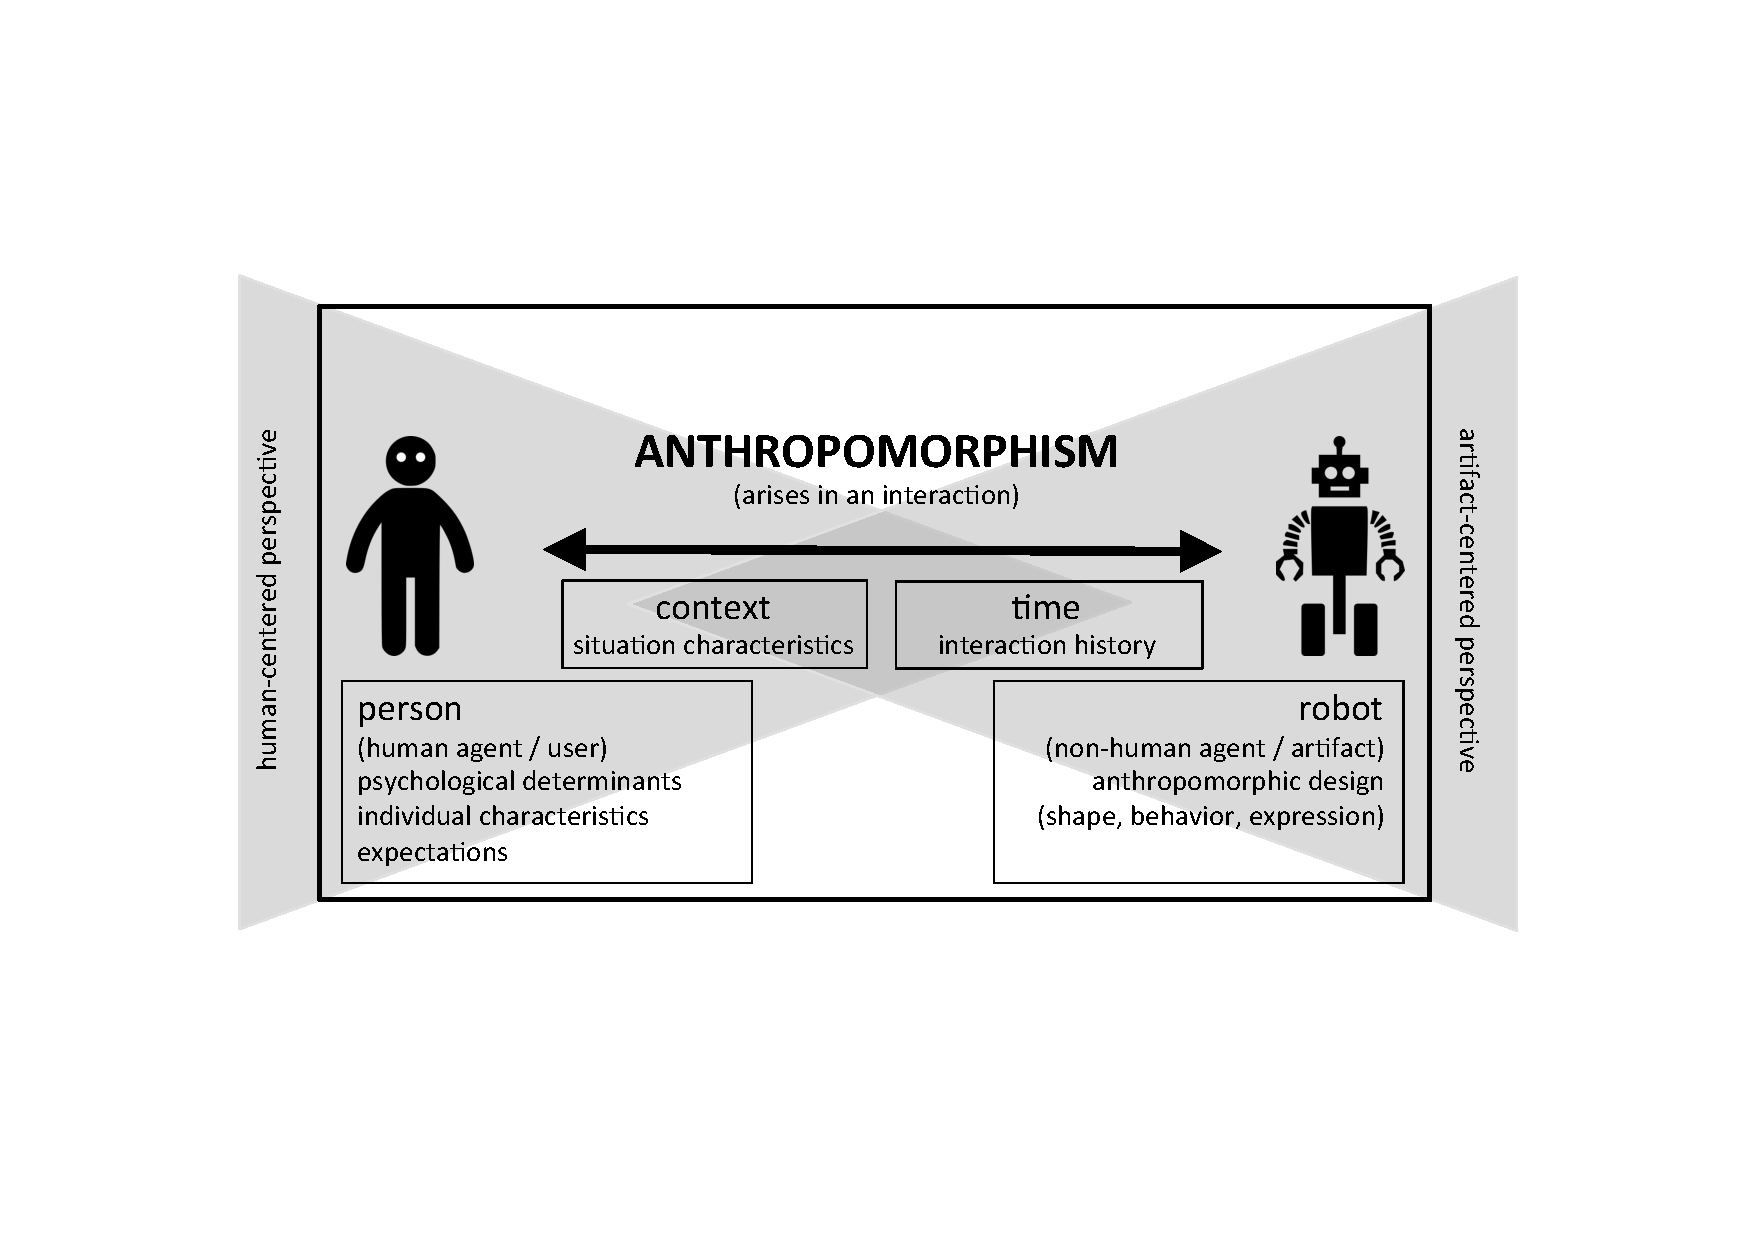
\includegraphics[width=0.75\columnwidth]{anthropo.pdf}
    \caption{Anthropomorphism is a multi-factor phenomenon. How far people tend
    to anthropomorphize a robot is determined by four main factors: the design
    of the robot $(R)$, the personal characteristics of the human user $(H)$, the
    situation and context in which the interaction occurs $(C)$, and the amount of
    time (repeated interaction) that the user spends to familiarize herself with the
    robot $(t)$.}

    \label{fig:anthropofig}
\end{figure}


Summing it up, and while anthropomorphism is a commonly discussed and studied
trait of human-robot interaction, its current understanding is somewhat limited:
when looking at understanding why anthropomorphism arises in an interaction
between a human and a non-human artifact, most attention is given to the
artifact itself. This is however not the full story, and when considering
anthropomorphism as a specific type of \textit{experience} that arises in an
\textit{interaction} between a set of user expectations and the external
reality~\citep{persson_anthropomorphism_2000}, it appears that complex human
factors, the interaction context, and the interaction history do play key roles.

It appears thus important to consider anthropomorphism as a phenomenon which is
determined by multiple factors, depicted on Figure \ref{fig:anthropofig}:

\begin{enumerate}

\item ~the characteristics of the \textbf{robot's design} (degree of
    anthropomorphic form),

\item ~the complex cognitive and psychological determinants of the \textbf{human
    user}~\citep{epley_seeing_2007},

\item ~the characteristics of the \textbf{context / situation} in which the
    interaction occurs, and

\item ~the fact of the user getting familiar with the robot \textbf{over time}
    (duration / history of interaction)

\end{enumerate}

As such, we use in the remaining of the article the notation \Ant[R,H,C,t] to
represent anthropomorphism as a function of the robot's traits $R$, the human
determinants $H$, the characteristics of the interaction context $C$ and the
history of the interaction itself, $t$. This last factor, time, is the focus of
the next section.

%%%%%%%%%%%%%%%%%%%%%%%%%%%%%%%%%%%%%%%%%%%%%%%%%%%%%%%%%%%%%%%%%%%%%%%%%
%
%
%
%				PART 2: OUR IDEAS -- A DYNAMIC PHENOMENON
%
%
%
%%%%%%%%%%%%%%%%%%%%%%%%%%%%%%%%%%%%%%%%%%%%%%%%%%%%%%%%%%%%%%%%%%%%%%%%%

\section{Anthropomorphism: a dynamic phenomenon}
\label{sec:our-ideas}

The HRI community has yet to investigate in depth the impact of time on
anthropomorphism. We already discussed how humans directly (more or less
mindlessly) respond to life-like and social cues emitted by non-human agents:
without thoughtful mental processing, humans tend to apply stereotypes and
heuristics to the robot, and in turn apply human-human social schemas and norms
to the occurring interactions. Following concepts introduced by
\cite{takayama_perspectives_2012}, we also mentioned how \emph{reflective}
interactions may succeed to \emph{in-the-moment} reactions, due to
\emph{familiarization} effects.

These dynamic modes of interactions reflect the changes in user
experience~\citep{karapanos_user_2009} and relationship to the robot, and are
given rhythm by specific interaction episodes like the \emph{novelty effect},
first pointed out by~\cite{kanda_interactive_2004}.

In the introduction, we reported on a few selected experimental results that
illustrate how the user tendency to anthropomorphize decreased over time.
Combined with the discussion on the nature and factors of anthropomorphism that
we proposed in section~\ref{sec:anthropomorphism}, we introduce in the following
section a novel qualitative model of the evolution of anthropomorphism over
time, \ie a model of the \emph{dynamics of anthropomorphism}.


\subsection{A Model of the Dynamics of Anthropomorphism}
\label{sec:dynamics-model}

To better structure the reflection about the interplay between anthropomorphism
and interaction history, we propose to introduce a phenomenological model of the
dynamics of anthropomorphism.  (Figure~\ref{fig:dynamics}, first presented
in~\citep{lemaignan2014dynamics}).  It represents how the level of
anthropomorphic \emph{effects}~\AntE[R,H,C,t] (\ie the observable manifestations
of the anthropomorphism \Ant) evolves over a long-term human-robot interaction.

While the model primarily considers \emph{long-term interaction} -- direct
(non-mediated), repeated interaction with the same robot, over an extended
period of time (typically longer than a week) --, we also introduce the
so-called \emph{novelty effect}~\citep{kanda_interactive_2004} that models the
first phase of human-robot interaction, during which a specific increase of
anthropomorphic interactions is observed.

In this model, anthropomorphism is quantified by a \emph{normalized level of
anthropomorphic effects} $\antENorm[R,H,C,t] = \frac{\antE[R,H,C,t]}{\antEMax}$:
because anthropomorphic effects are often qualitative and difficult to quantify
on an absolute scale, the model represents them as a normalized value, that
spans from a minimum (no anthropomorphic effects: $\antE=0$) to a maximum
(\AntEMax, with $t_{max} = \operatorname{arg\,max}_t \, \antE[t]$, which we
hypothesize to correspond to the novelty effect ``peak''). For the sake of
readability, we will use \AntE in the following sections to refer to the
normalized level of anthropomorphic effects.

While not the focus of this article, we discuss in section~\ref{sec:measuring}
some of the possible methodologies and techniques for the quantitative and
qualitative assessment of anthropomorphic effects.

\begin{figure*}[htb]
\centering


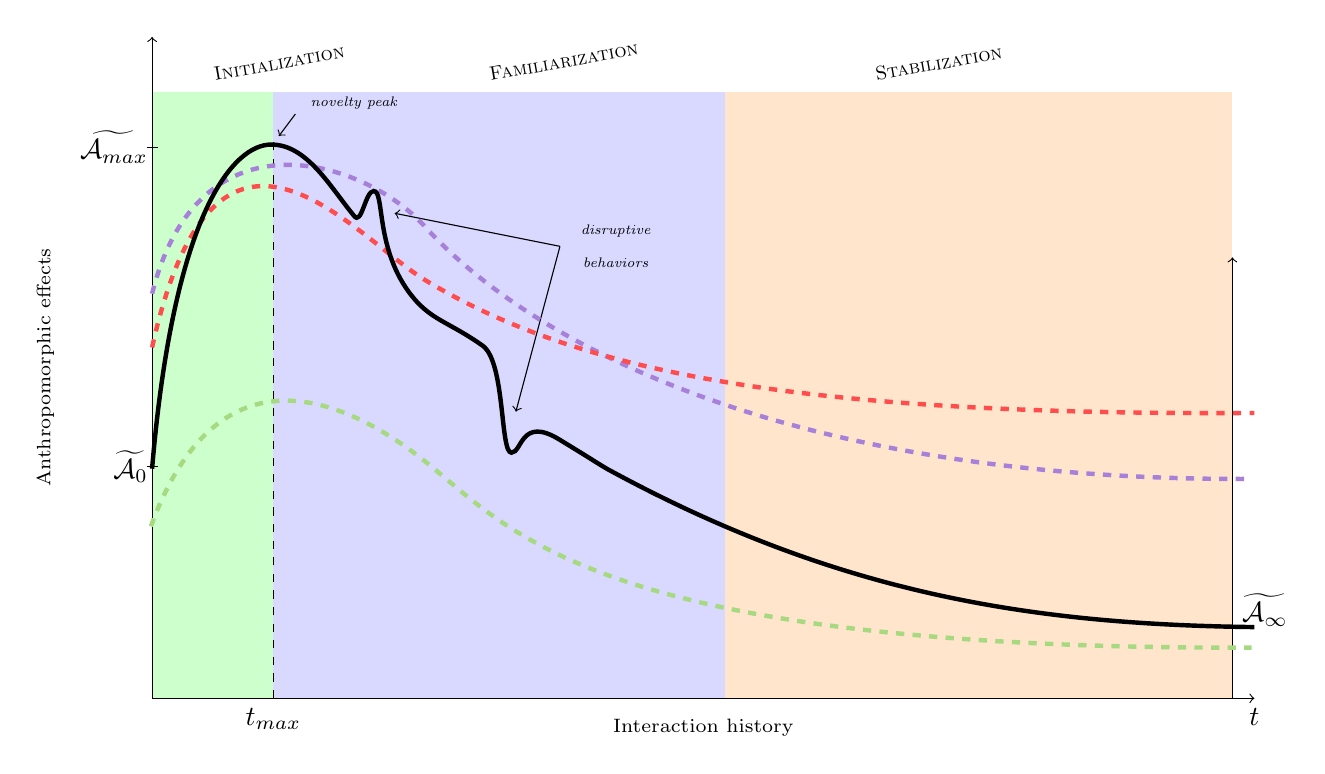
\begin{tikzpicture}[scale=1.4]

% background shading
\path[fill=green!20] (0,0) rectangle (1.1,5.5);
\path[fill=blue!15] (1.1,0) rectangle (5.2,5.5);
\path[fill=orange!20] (5.2,0) rectangle (9.8,5.5);
\draw(0.5,5.5) node[anchor=south west, rotate=10] {\scriptsize \sc Initialization};
\draw(3,5.5) node[anchor=south west, rotate=10] {\scriptsize \sc Familiarization};
\draw(6.5,5.5) node[anchor=south west, rotate=10] {\scriptsize \sc Stabilization};
% horizontal axis
\draw[->] (0,0) -- (10,0) node[anchor=north] {$t$};
\draw(5,-0.1) node[anchor=north] {\scriptsize Interaction history};


% vertical axis
\draw[->] (0,0) -- (0,6) node[anchor=east] {};
\draw(-0.8,3) node[rotate=90,anchor=south] {\scriptsize Anthropomorphic effects};

\draw (-0.05, 2.1) -- (0.05, 2.1) node[anchor=east] {\IPAe};
\draw (-0.05, 5) -- (0.05, 5) node[anchor=east] {\AntEMax};

% vertical axis - end
\draw[->] (9.8,0) -- (9.8,4) node[anchor=east] {};
\draw (9.8, 0.8) node[anchor=west] {\SLAe};


\draw[<-] (1.15,5.1) -- (1.30,5.3) node[anchor=east] {};
\draw (1.35,5.4) node[anchor=west] {\tiny \it novelty peak};

\draw[dashed] (1.1, 0) -- (1.1,5.1);
\draw (1.1,0) node[anchor=north] {$t_{max}$};

%\draw[dotted] (0, 5) -- (6.2,5);
%\draw[dotted] (0, 3) -- (6.2,3);
%\draw[<->] (6.1,3) -- (6.1,5) node[sloped, above, midway] {$\Delta_{a}$};

\draw[<-] (2.2,4.4) -- (3.7,4.1) node[anchor=east] {};
\draw[<-] (3.3,2.6) -- (3.7,4.1) node[anchor=east] {};
\draw (3.8,4.1) node[anchor=west, align=center] {\tiny \it disruptive\\ \tiny
\it behaviors};
%%%%%
%% CURVES
%%%%
\begin{scope}[yscale=-1,shift={(-0.125,-0.46)}]
    \draw[ultra thick, green!70!red!50, dashed] svg[scale=1cm] "M 0.114,-1.1 C 0.733,-2.79 1.88,-2.23
    2.51,-1.76 3.34,-1.14 3.94,0.02 10.1,0";

    \draw[ultra thick, blue!70!red!50, dashed] svg[scale=1cm] "M 0.125,-3.21 C 0.549,-4.91 2.05,-4.42
    2.59,-3.83 3.57,-2.74 5.93,-1.51 10.1,-1.53";

    \draw[ultra thick, red!70, dashed] svg[scale=1cm] "M 0.12500001,-2.7222489 C 0.70533638,-5.3401235 1.9431386,-3.7307246 2.608741,-3.3299187 c 1.3619528,0.8201274 3.3166657,1.2251393 7.515191,1.2014756";

    \draw[ultra thick] svg[scale=1cm] "M
    0.125,-1.622832 c 0.19887378,-2.35086 0.74751962,-2.9373641 1.0765913,-2.9404859 0.3290717,-0.00312 0.5370891,0.383599 0.754419,0.6452353 0.069872,0.099803 0.1021612,-0.2231749 0.1792538,-0.2238964 0.099707,0 0.013454,0.4985362 0.3173383,0.9139831 0.1911917,0.2612926 0.3444354,0.2578391 0.6711932,0.4894291 0.2058265,0.1458798 0.1571532,0.9762306 0.2615031,0.9702183 0.097182,0 0.083295,-0.3336208 0.4330446,-0.1199242 0.4306401,0.2631203 0.216699,0.1355642 0.4296663,0.2647074 2.0858202,1.13836043 3.8496455,1.41300027 5.8769904,1.43753027";



\end{scope}

\end{tikzpicture}

\caption{\textbf{Qualitative model of the dynamics of anthropomorphism}. We
    distinguish three main phases: \emph{initialization}, \emph{familiarization}
    and \emph{stabilization}, preceded by a \emph{pre-interaction} phase. The
    pre-interaction phase is characterized through an \emph{initial potential to
    anthropomorphize} (IPA, noted \IPAe).  Once the interaction starts, the level
    of anthropomorphism increases, in part due to the \emph{novelty effect}, and then
    decreases to reach a \emph{stabilized level of anthropomorphism} (SLA, noted
    \SLAe). \IPAe and \SLAe may vary depending on the user (and his/her
    expectations), the robot and the context of interaction.  During the
    interaction, unpredicted behaviors of the robot (\emph{disruptive
    behaviors}) may lead to local increases or decreases of the level of
    anthropomorphic effects. The duration of these phases may vary and the
    overall shape of the curve is unique to each human interacting with a
    specific robot in a given context, as emphasized by the alternative curves.}

\label{fig:dynamics}
\end{figure*}

\subsection{Three phases}
\label{sec:phases}

We distinguish three main phases that describe the evolution of the
anthropomorphic effects in a long-term human-robot interaction. They are
depicted in different shades in Figure~\ref{fig:dynamics}.

\subsubsection{Pre-Interaction and Initialization Phase\\}

The \emph{initial potential to anthropomorphize} \IPAe describes the initial
potential for the human user to anthropomorphize the robot in a given situation.
This potential depends on the several factors introduced in
section~\ref{sec:multi-factors}.  It represents the level of anthropomorphic
effects that can be expected to occur during the very first contacts between the
human and the robot. During this first phase, pre-conceptions and initial
expectations as well as previous experience of the user with other similar types
of robots and similar contexts are of prime importance.

During the initialization phase, we expect an increasing value of \Ant that is
due to the effects of the novelty of the robot. Such effects have been described
with interactive technologies in general \citep{rogers_diffusion_1995}, and also
in several long-term HRI studies in workplaces
\citep{huttenrauch_fetch-and-carry_2003,mutlu_robots_2008}, in schools and
public places
\citep{gockley_designing_2005,kanda_communication_2005,kanda_interactive_2004},
and elder care centers \citep{sabelli_conversational_2011}. Also long-term
studies of domestic robots have shown similar effects -- and also found that
after some time people's interest, engagement, and fascination of the robot
decreased
\citep{sung_robots_2009,sung_domestic_2010,fernaeus_how_2010,fink_living_2013}.

The type of anthropomorphic effects typically observed during the initialization
phase include users who spontaneously tend to talk directly to the robot while
they are aware that the system is not be able to recognize speech (greeting the
robot, asking questions to it, giving it a nickname, praising the robot,
commenting on its performances, giving commands), the use of pointing gestures
and waving at the robot, as well as ascribing gender and some personal
preferences or intention to the robot.

\subsubsection{Familiarization Phase\\}

In this context, \emph{familiarization} means \emph{to get acquainted with}.
It is not to be confused with the \emph{familiarity thesis} that relates to the
projection of already known cognitive models onto the robot. We discuss this other
aspect in section~\ref{sec:cognition-neuroscience}.

The \emph{familiarization phase} starts at the peak of the \emph{novelty
effect}: anthropomorphic effects are at their maximum, the user thinks (s)he is
potentially facing an agent aiming at ``human-level intelligence'' (to take
McCarthy's words). This is a transient state that quickly vanishes, and the
projected anthropomorphism then starts to decrease while the human observes and
recognizes that the behavior of the robot is generally \emph{predictable} and
possibly \emph{deceptive} (for instance, it talks but does not understand when
we talk; it has eyes but does not recognize everyday objects we show; \etc).

\paragraph{Disruptive behaviors.}

We call \emph{disruptive behaviors} any behavior exhibited by the robot that
appears unexpected to the user: for instance, a robot may usually follow always
the same route to go from one place in a house to the other, but suddenly it
might change the route. The actual underlying reason may span from a bug to the
detection of a new obstacle, but as long as this reason is not immediately
intelligible to the user, the behavior counts as \emph{disruptive}. We further
discuss the role of disruptive behaviors in cognitive terms in section
\ref{sec:disruptive}.


\subsubsection{Stabilization Phase\\}

During the \textit{Stabilization Phase} the value of \Ant tends to stabilize over
a longer time, to reach a value that we call the \textit{Stabilized Level of
Anthropomorphism} (SLA), noted \SLAe. The value that the
SLA approaches is unique for each user interacting with a specific robot in a
given situation. \SLAe may approach $0$, when no anthropomorphic effects
are observed anymore, for instance when the user is interacting with the robot
in a routine way and he/she does not project any human-like traits unto the
robot, what \cite{takayama_toward_2011} calls the robot being
\textit{``invisible in use''}. \SLAe may as well remains above 0 if the user
continues to exhibit anthropomorphic behaviors when interacting with the robot
on the long run.

The level \SLAe, like \IPAe, is the result of a combination of multiple human,
robotic and contextual factors, with the additional impact of the
\emph{interaction history t} that the user experienced with the robot. Note that
the IPA and SLA levels are generally not correlated: a person may initially
have a high potential of anthropomorphizing (high \IPAe), for instance a highly
anthropomorphic robot, but subsequently get disappointed by the actual
capabilities of it and stop explaining it in terms of human-like characteristics
(low \SLAe). Another user may however create lasting affective bonds with the
same robot and may continue to anthropomorphize the robot (higher \SLAe).



%%%%%%%%%%%%%%%%%%%%%%%%%%%%%%%%%%%%%%%%%%%%%%%%%%%%%%%%%%%%%%%%%%%%%%%%%
%
%
%
%		PART 3: EXPLANATIONS -- COGNITIVE CORRELATES, NEUROSCIENCE VIEW
%
%
%
%%%%%%%%%%%%%%%%%%%%%%%%%%%%%%%%%%%%%%%%%%%%%%%%%%%%%%%%%%%%%%%%%%%%%%%%%

\section{Towards a Cognitive Interpretation}
\label{sec:cognition-neuroscience}

The model that we have introduced so far helps to represent and organize the
\emph{observations} of anthropomorphism. It does so at a conceptual level, and
with a special emphasis on the evolution over time.

This abstract model may contribute to a better understanding of the
\emph{phenomenology} of anthropomorphism, but it does not help to \emph{explain}
the phenomenon. This section proposes to look at the dynamics of
anthropomorphism in terms of \emph{cognitive correlates}: how human cognition
can explain the dynamic nature of our interactions with robots, and what are the
main cognitive layers upon which researchers can build to design better, deeper
human-robot interactions.

We also discuss two specific aspects: the cognitive impact of disruptive
behaviors (section~\ref{sec:disruptive}) on mutual modeling, and how our models
relate to the \emph{in-the-moment} versus \emph{reflective} perspectives on
agency in HRI~\citep{takayama_perspectives_2012}.


\subsection{A Model of the Cognitive Layers of Human-Robot Interaction}
\label{sec:cognitive-model}


\begin{figure}[htb]
\centering
%\resizebox{\linewidth}{!}{
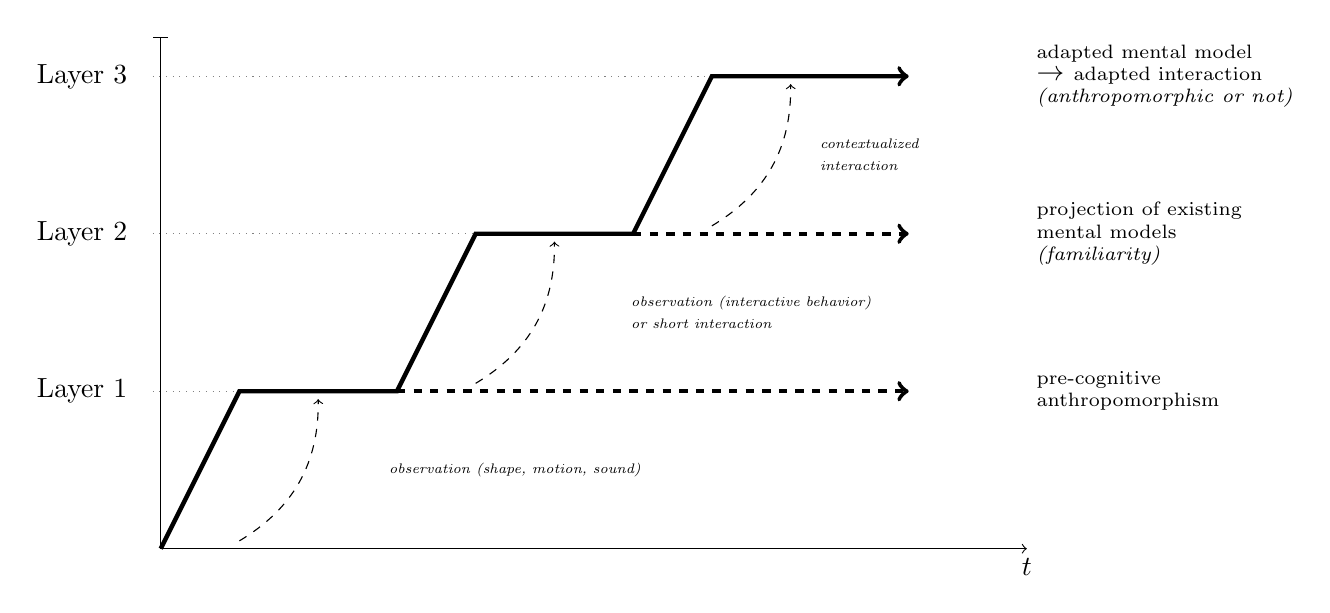
\begin{tikzpicture}
\baselineskip=8pt

%\path[fill=gray!20] (0,0) rectangle (10.5,2);
%\path[fill=gray!50] (0,2) rectangle (10.5,4);
%\path[fill=gray!20] (0,4) rectangle (10.5,6);

\draw (-0.3,2) node[anchor=east] {Layer 1}
      (-0.3,4) node[anchor=east] {Layer 2}
      (-0.3,6) node[anchor=east] {Layer 3};

\draw[thin,black!50,dotted] (-0.10,2) -- (1,2);
\draw[thin,black!50,dotted] (-0.10,4) -- (4,4);
\draw[thin,black!50,dotted] (-0.10,6) -- (7,6);

\draw[->] (0,0) -- (11,0) node[anchor=north] {$t$};
\draw[-|] (0,0) -- (0,6.5) node[anchor=east] {};
% Us
\draw[ultra thick, ->] (0,0) -- (1,2) -- (3,2) -- (4,4) -- (6,4) -- (7,6) --
(9.5,6);
\draw[ultra thick, dashed, ->] (3,2) -- (9.5,2);
\draw[ultra thick, dashed, ->] (6,4) -- (9.5,4);

\draw (11,2) node[align=left, anchor=west]{\scriptsize pre-cognitive\\\scriptsize anthropomorphism}; %label

\draw (11,4) node[align=left, anchor=west] {\scriptsize{projection of existing}\\\scriptsize{mental models}\\\scriptsize{\it (familiarity)}}; %label

\draw (11,6) node[align=left, anchor=west] {\scriptsize{adapted mental
model} \\ $\to$ \scriptsize{adapted interaction}\\\scriptsize{\it (anthropomorphic or not)}}; %label


\draw[dashed,->] (1,0.1) to[bend right] (2,1.9)  node at (4.5,1) {\tiny{\it observation (shape, motion, sound)}}; %label

\draw[dashed,->] (4,2.1) to[bend right] (5,3.9)  node[align=left] at (7.5,3) {\tiny \it observation (interactive behavior) \\ \tiny \it or short interaction}; %label

\draw[dashed,->] (7,4.1) to[bend right] (8,5.9)  node[align=left] at (9,5)
{\tiny \it contextualized\\ \tiny \it interaction}; %label

\end{tikzpicture}
%}
\caption{\textbf{The three cognitive layers of anthropomorphism}: Layer 1 is the instinctive,
sub-cognitive identification of living peers. {\it Empathy} is characteristic
of this stage. After longer observation or short, non-contextualized interaction
(typically, a lab environment), the user enters Layer 2: the user projects a
mental model he/she is already familiar with onto the robot. After longer {\it
contextualized} interaction (typically, at home), the user enters Layer 3 of
anthropomorphism: the user composes a custom mental model of the robot,
based on experience. This leads to adapted interaction modalities, that may
still be anthropomorphic, or not. Note that the different layers coexist: Layer
1 and 2 still affect the human perception of the robot in a Layer 3 interaction.}
\label{fig:cognitivemodel}
\end{figure}

We propose three different cognitive layers (Figure~\ref{fig:cognitivemodel}),
which are not mutually exclusive but overlap over time. Note that these three
cognitive stages are related but do not exactly match the \emph{Initialization},
\emph{Familiarization} and \emph{Stabilization} phases introduced in our model
of the dynamics of anthropomorphism. We discuss this relation hereafter.

The main underlying cognitive process in anthropomorphism is understood as
perceiving and reasoning about something non-human and unfamiliar based on one's
representation of the familiar and well-known concept of being
human~\citep{epley_when_2008}. This led us to interpret the phases of
anthropomorphic interactions as parallel cognitive phases
(Figure~\ref{fig:cognitivemodel}).

The \emph{Layer 1} is the instinctive, pre-cognitive identification of living
peers. Studies conducted by~\citet{rosenthal-vonderputten_experimental_2013},
who investigated the neural correlates of emotional reactions of humans towards
a robot, supports the idea that humans tend to anthropomorphize robots
intuitively in this pre-cognitive way. {\it Empathy} is characteristic of this
layer~\citep{rosenthalvonderPutten2013neural}.  It is also at this stage that
automatic activation of the human's mirror neurons system  in response to
viewing the robots action and human automatic emotional responses are
contributing at a lower level to the intuitive anthropomorphization.

The intuitive anthropomorphization in the cognitive Layer 1 might be
characteristic of what \cite{takayama_perspectives_2012} calls the
\textit{in-the-moment} perspective on agency with a robot compared to the
\textit{reflective} perspective (see paragraph ``artifact-centric perspective''
in section \ref{sec:anthropomorphism}).  For instance, we reflectively might
\textit{not} perceive agency in a social robot, but it can feel quite
differently in the moment of interaction. \cite{takayama_perspectives_2012}
argues that neglecting to separate reflective perspectives from in-the-moment
perspectives of agency is one of the major sources of confusion when people talk
and write about anthropomorphism. There seems to be a disconnection between what
people consciously perceive and how they respond to stimuli that they may not
consciously perceive. This means that in the initial phase of interacting with a
novel device \textit{(initialization)} (see Figure \ref{fig:dynamics}) people
might not respond consciously but rather mindlessly \citep{nass_machines_2000},
and in turn anthropomorphize more. They start to respond in a more reflective
manner only during the \textit{familiarization} (in turn, the tendency to
anthropomorphize might decrease). This can be illustrated by the fact that
people tend to deny interacting with computational systems as if they were
people and yet they respond to computers in many ways that are remarkably
similar to how they respond to people \citep{reeves_media_1996}.
\cite{takayama_perspectives_2012} also applies a cognitive viewpoint on the two
different perspectives of in-the-moment \vs reflective to illustrate
differences. She states that in-the-moment perceptions of agency are largely
shaped by bottom-up perceptual processes, evoking very immediate responses (\eg
to the cues emitted by the artifact's design (``artifact-centric
perspective''). In contrast, according to Takayama, reflective perceptions are
more often shaped by top-down processes because of the nature of reflective
thought.

After a longer observation period (typically including complete action sequences
of the robot) or short interaction (touching, short talk like greetings), we
suggest the human activates the cognitive \emph{Layer 2}: in this phase, the human
starts building a behavioral and cognitive model of the robot that would support
both the observed and imagined capabilities of the robot.  The \emph{familiarity
thesis}~\citep{hegel_understanding_2008} supports the idea that the human first
projects onto the robot mental models of similar agents he/she is already
familiar with (ranging from animals to human adults, to pets and children). We
hypothesize that the nature of the projected mental model, as well as how deep
the human engages in this projection, might be driven by the same parameters as
we mentioned for the \emph{initial potential to anthropomorphize}. We also believe
that, at this stage, the human also changes his attitude towards the robot, by
focusing his attention to social cue more than to low-level behaviors, which
may in turn reinforce the resonance mechanisms.

The cognitive \emph{Layer 3} is gradually activated after a
\emph{contextualized} interaction.  A \emph{contextualized} interaction is
\emph{explicitly purposeful} (the purpose of the interaction, be it purely
entertainment, is explicit and conscious to the human), and takes place in an
environment that fosters a stronger cognitive (and possibly affective/social)
commitment from the human in the interaction (typically, at home). During this
interaction, the human iteratively restates and reshapes his/her behavioral and
mental model of the robot (\emph{How does the robot react to such and such
situation/input?  What does the robot know about me? About itself? About our
environment? What can the robot learn?}, etc.).

\begin{figure}[]
\centering
%\resizebox{\linewidth}{!}{
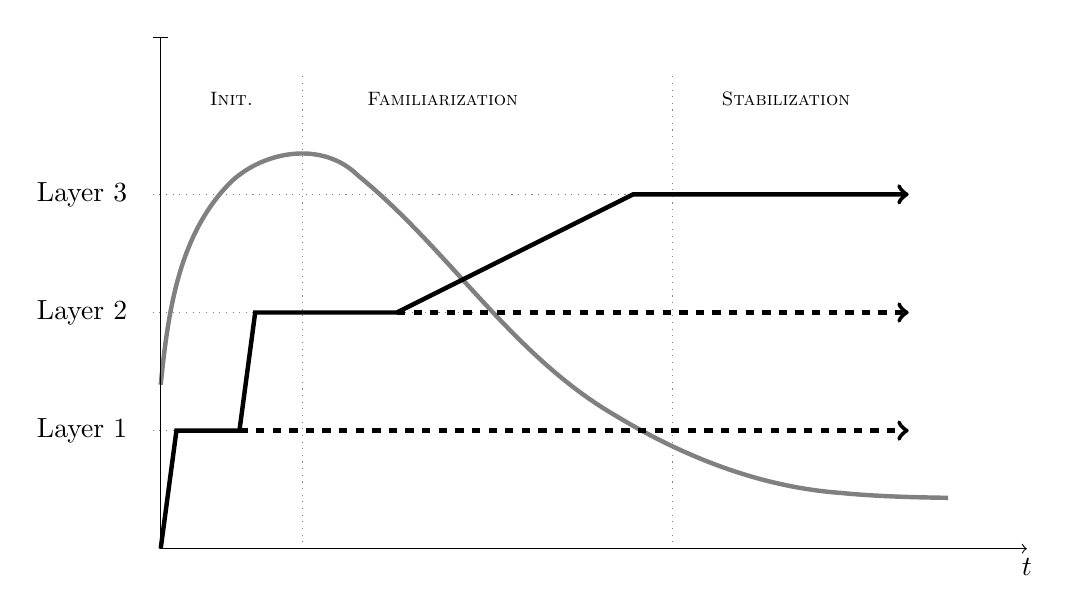
\begin{tikzpicture}
\baselineskip=8pt

\draw[dotted, black!50, thin] (1.8, 6) -- (1.8, 0);
\draw[dotted, black!50, thin] (6.5, 6) -- (6.5, 0);

\draw(0.5,5.5) node[anchor=south west] {\scriptsize \sc Init.};
\draw(2.5,5.5) node[anchor=south west] {\scriptsize \sc Familiarization};
\draw(7,5.5) node[anchor=south west] {\scriptsize \sc Stabilization};


\begin{scope}[yscale=-1,shift={(-0.125,-0.46)}]
    \draw[ultra thick, black!50] svg[scale=1cm] "M 0.125,-1.622832 c 0.093536,-0.9062795
    0.21996726,-1.9131565 0.9017912,-2.5842389 0.4277536,-0.3944265
    1.1653486,-0.5108382 1.605386,-0.071103 1.1558512,0.9403904
    1.9535208,2.2825896 3.2616057,3.0430907 0.871821,0.52801518
    1.8461798,0.91299355 2.8702084,0.98695145 0.4522402,0.0444213
    0.9069132,0.0552179 1.3610087,0.0620963";

\end{scope}

\draw (-0.3,1.5) node[anchor=east] {Layer 1}
      (-0.3,3) node[anchor=east] {Layer 2}
      (-0.3,4.5) node[anchor=east] {Layer 3};

\draw[thin,black!50,dotted] (-0.10,1.5) -- (1,1.5);
\draw[thin,black!50,dotted] (-0.10,3) -- (4,3);
\draw[thin,black!50,dotted] (-0.10,4.5) -- (7,4.5);

\draw[->] (0,0) -- (11,0) node[anchor=north] {$t$};
\draw[-|] (0,0) -- (0,6.5) node[anchor=east] {};
% Us
\draw[ultra thick, ->] (0,0) -- (0.2,1.5) -- (1,1.5) -- (1.2,3) -- (3,3) -- (6,4.5) --
(9.5,4.5);
\draw[ultra thick, dashed, ->] (1,1.5) -- (9.5,1.5);
\draw[ultra thick, dashed, ->] (3,3) -- (9.5,3);

\end{tikzpicture}
%}
\caption{\textbf{Towards a cognitive interpretation of the dynamics of
    anthropomorphism}: This diagram combines the figures~\ref{fig:dynamics}
    and~\ref{fig:cognitivemodel} to evidence their interplay: we suggest that
    the cognitive stages 1 and 2 (pre-cognitive anthropomorphism and projection
    of known existing cognitive models) first play a key role in the early
    perception of the robot, leading to high levels of anthropomorphic
    behaviors. Then, the user smoothly transitions from projecting already known
    models to building a new, specific cognitive model of the robot: this occurs
    while the user familiarizes with the robot and leads over time to a
    stabilized level of anthropomorphic behaviors. In the current state of
    robotic technology, this stabilization mostly reads as a \emph{decrease} of
    anthropomorphic perception, due to the user being able to explain and
    accurately predict the robot behavior after enough interaction time, hence
    perceiving the robot as a simple machine.}

\label{fig:mix}
\end{figure}


This mental process depends on the human understanding of the robot's inner
working, as well as his/her own tendency to anthropomorphize (the
\emph{personality} in IPA factor). At this stage, the \emph{perception} of the
robot (its shape for instance) and its original intended \emph{purpose} play
less of an important role. It is mostly a human-centric process.  The result of
this third phase is an iteratively adapted cognitive model of the robot.

Another way to think of the three proposed cognitive stages is to relate them to
the \textbf{user experience} which is characteristic of these three stages. For
instance, \cite{norman_emotional_2003} characterizes  three user experience
dimensions (related to emotional attachment), which occur when people use or see
a product for the first time: \emph{(1)} the \emph{visceral level}, which is the
first impression of a product based on its experience; at this level people do
not think about a product but make spontaneous judgments; \emph{(2)} the
\emph{behavioral level}, in which people use and experience the product,
appraise its functions, and consider aspects such as usefulness and usability;
\emph{(3)} the \emph{reflective level}, in which consciousness takes part in the
process, and past experiences are taken into account.

\subsection{Relation to the dynamics of anthropomorphism}

As mentioned before, the three cognitive stages proposed here do not directly
match with the three phases in the model of the dynamics of anthropomorphism,
and Figure~\ref{fig:mix} attempts to depict their interplay.
The cognitive Layers 1 and 2, in particular, are both active in the
\emph{initialization} phase of the anthropomorphism model. Sub-cognitive
anthropomorphism typically \emph{initiates} the novelty effect by rapidly
engaging the human in the interaction through an initial projected agency,
whereas cognitive Layer 2 (projection of familiar mental models) supports the
novelty effect by inducing beliefs that the robot is set up with possibly
complex cognitive abilities.

The cognitive Layer 3 also overlaps with the \emph{Familiarization} phase: as
the human gets used to the robot, he/she restates and adapts its
cognitive model of the robot by iteratively reshaping pre-existent, familiar
models until it provides a satisfying support to explain and justify the
observed robot behavior.

A \emph{stable level of anthropomorphism} is reached when the adaptation process
depicted in the cognitive Layer 3 reached a stable state, \ie the user's
experience with the robot is correctly supported by the cognitive model he/she
has built.


\subsection{Role of unexpected behaviors}
\label{sec:disruptive}

A cognitive interpretation of anthropomorphism also allows to better interpret
the role of unexpected robot behaviors, that are \emph{disruptive} with respect
to the cognitive process of building a mental model of the robot.

Common observation of naive people (children or adults) interacting with robots
shows that unexpected behaviors of the robot can have a notable impact on
interaction. This is supported by the results from~\citet{Waytz2010}, mentioned
in section \ref{sec:cognitive-expl}, that show that people attribute more easily
anthropomorphic features to artifacts when they have unpredictable behaviors.
Also \cite{short_no_2010} found that variations in a robot's behavior (such that
it is unexpected) influence people's attribution of mental states and
intentionality to a robot. Participants who were playing the
``rock-paper-scissors'' game with a robot that tried to cheat (either verbally
or in its action), displayed a greater level of social engagement and made
greater attributions of mental states, and conversely, unexpected robot
behavior, when interpreted as a robot failure, has been observed to adversely
affect cognitive engagement: \cite{desai_impact_2013}, for instance, found that
in an interaction scenario, early failures of the robot can cause a dramatically
lower real-time trust.

Accordingly, we suggest that unexpected robot behaviors lead the user to restate
his/her behavioral model, and hence, his/her cognitive model of the robot, which
translates into an increase or decrease of the level of anthropomorphism
(depicted by the spikes in Figure~\ref{fig:dynamics}, p.~\pageref{fig:dynamics}).

When talking about \emph{unexpected robot behaviors}, several distinct cases can
be considered, summarized in Table~\ref{fig:perceptionUnexpectedBehavior}.

\begin{figure}
    \centering
    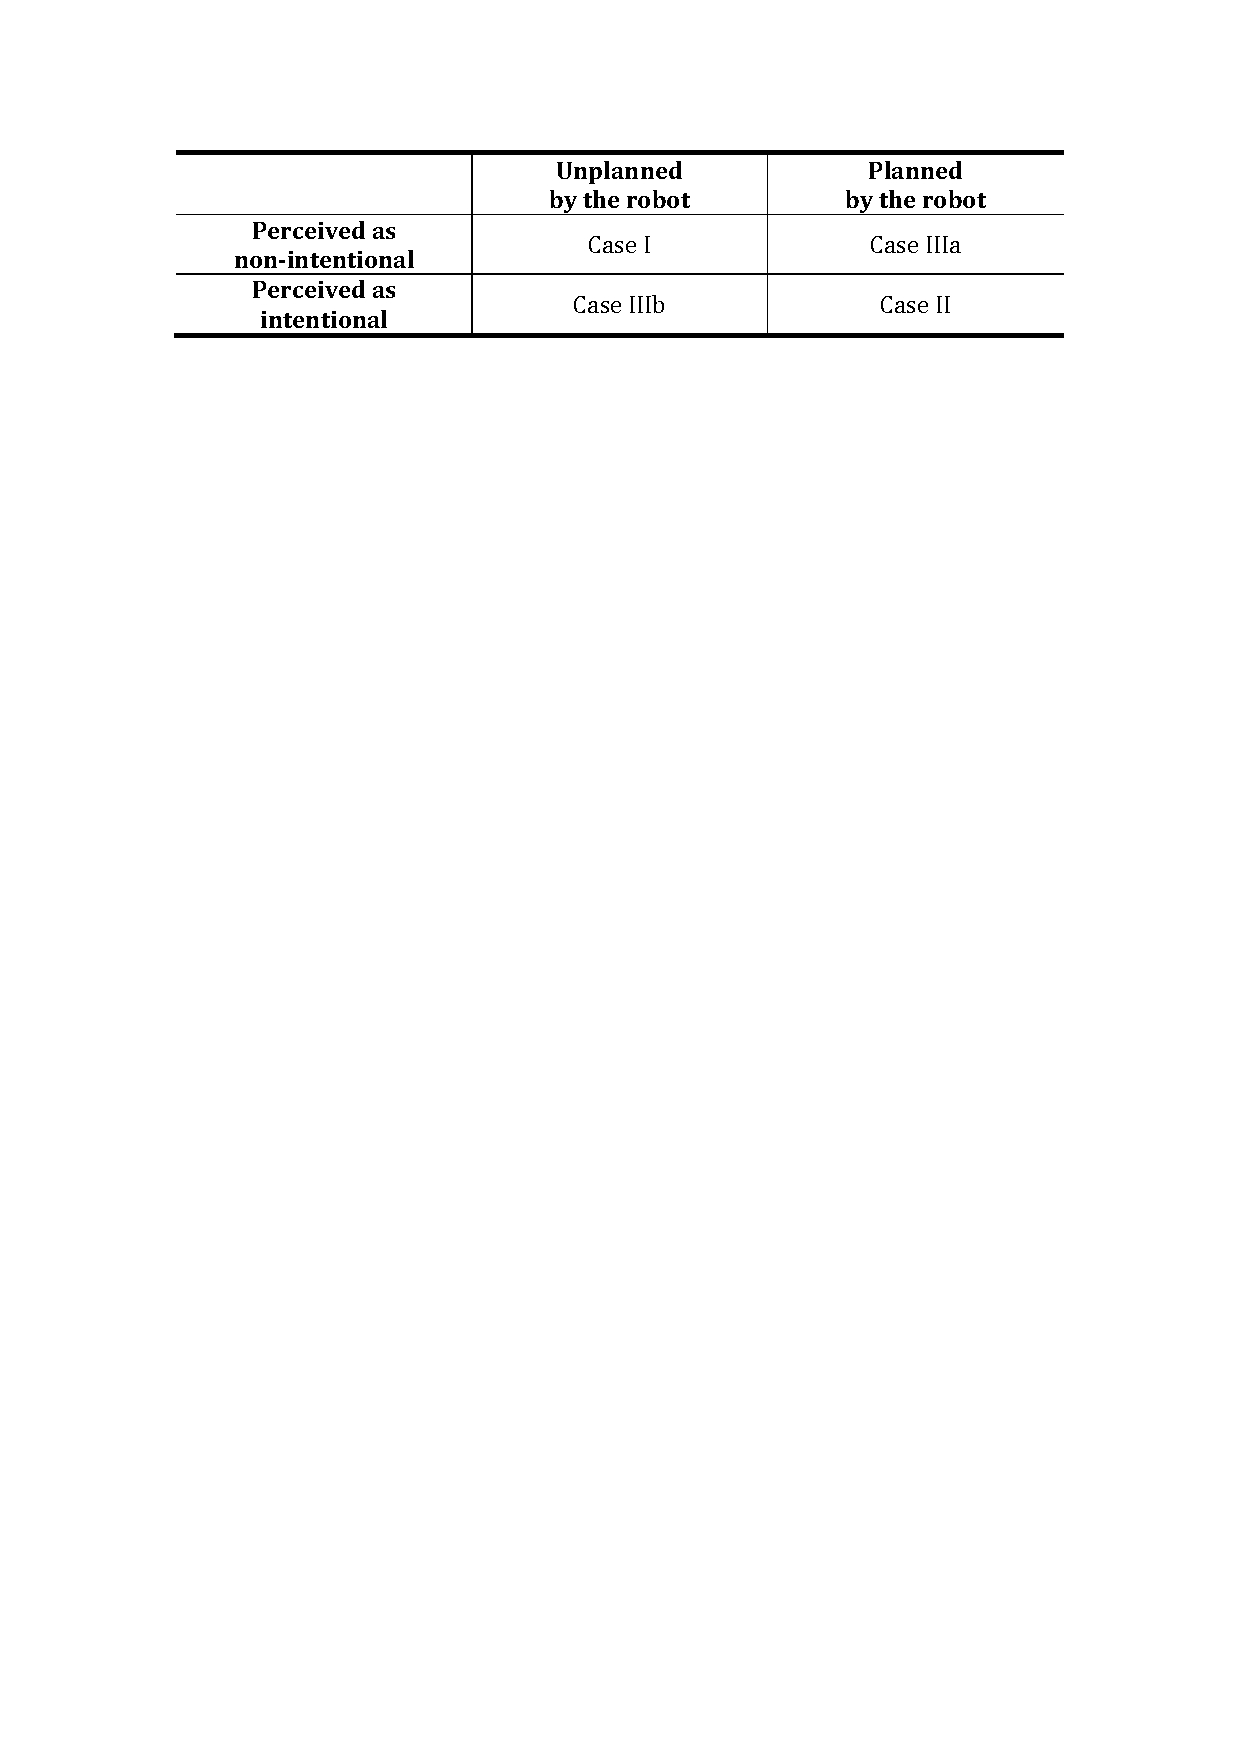
\includegraphics[width=0.75\columnwidth]{un-expected-behavior.pdf}
    \caption{Behaviors of the robot that are unexpected by the user may be intentional
    (the robot has planned the behavior) or not (typically, a failure:
    misdetection, bug,...). Independently of that, the behavior may be
    \emph{perceived} by the user as intentional or not.}

    \label{fig:perceptionUnexpectedBehavior}
\end{figure}


If the unexpected behavior is not planned, and perceived as such by the human
(case I, Table~\ref{fig:perceptionUnexpectedBehavior}), the human can interpret
that the robot is able to fail. If the robot explicitly states its failure (for
instance, by saying ``I'm lost!''), the behavior is then called
\emph{transparent}~\citep{kim_who_2006}, and suggests that the
robot has \emph{introspective} capabilities (it can reflect on its own internal
state), which may lead to higher anthropomorphic projections.  On the contrary,
if the robot shows no sign of recognizing its own failure, the user may ascribe
a lower level of anthropomorphism to the robot.

In case II, the robot voluntary executes a behavior that is unexpected by the
human, and the human perceives it rightfully as an \emph{intentional} behavior.
For instance, the human asks the robot to go somewhere, and the robot refuses,
saying ``I do not want to go there''. In that case, we expect to see an increase
of attribution of anthropomorphism due to the human ascribing intentionality to
the robot.

Case IIIa and IIIb correspond to misinterpretations of the robot behavior. Case
IIIb may actually lead to an increased level of anthropomorphism since the human
will (wrongfully) attribute intentionality to the robot, while case IIIa is
expected to lead to a lower anthropomorphism level.

%%%%%%%%%%%%%%%%%%%%%%%%%%%%%%%%%%%%%%%%%%%%%%%%%%%%%%%%%%%%%%%%%%%%%%%%%
%
%
%
%				CONCLUSIONS
%
%
%
%%%%%%%%%%%%%%%%%%%%%%%%%%%%%%%%%%%%%%%%%%%%%%%%%%%%%%%%%%%%%%%%%%%%%%%%%

\section{Conclusion}
\label{sec:conclusion}

In this paper, we have provided a broad account of the cognitive and
psychological viewpoints on anthropomorphism, with a novel focus on the
impact of time. Considering anthropomorphism as a social phenomenon that arises
in an interaction, we formulated the following three suggestions:

\begin{enumerate}

\item \textbf{Anthropomorphism is based on multiple factors.} The three main
    factors that constitute anthropomorphism are the characteristics of the
    human, the characteristics of the robot, and the characteristics of the
    context of use. A temporal dimension is taken into account by the
    \textit{interaction history} $t$, which reflects the fact that
    anthropomorphism is also a dynamic phenomenon.

\item \textbf{Anthropomorphism is dynamic.} Looking at how experience and
    interaction evolve over time, we developed a qualitative model of the
    dynamics of anthropomorphism, which materializes a non-linear relationship
    between the observable \textit{anthropomorphic effects} \AntE of the human
    behavior and the \textit{interaction duration} $t$ (the actual time the user
    has spent interacting with the robot for real or imagined). This qualitative
    relationship starts at $t_{0}$ with the \textit{initial potential to
    anthropomorphize} (IPA), a function of the three factors previously
    discussed (point 1) that measures a pre-interaction form of
    anthropomorphism. On the other end, at $t_{\infty}$, we suggest that the
    interaction reaches a \textit{stabilized level of anthropomorphism} (SLA).
    How the curve evolves in between these two values is flexible and unique to
    each user, robot, and context. We however generally hypothesize an increase of
    \textit{anthropomorphic effects} driven by the \textit{novelty} of the
    robot, followed by a decrease of \AntE as the user \textit{familiarizes}
    him/herself with the robot and with using the robot. 

\item \textbf{Anthropomorphism is multi-layered cognitive mechanism.} We have
    identified three successive and overlapping cognitive layers that underlie
    human-robot interaction and shape anthropomorphic behaviors.
    These layers (that are likely continuum rather than discrete levels) depend
    on one how typically human the robot is perceived, and how much the mental
    model that the user builds of the robot overlaps (or is inspired by) the
    mental model he/she has of another human. Each of the layers
    reflect different depths of cognitive engagement between the human and the
    robot.

\end{enumerate}

We believe that this systematic approach of anthropomorphism as a complex social
and psychological phenomenon, along with the terminology clarification that we
have proposed in the introduction of the article, can effectively support
further research on the intricate interactions between humans and robots.

We purposefully kept this work at a rather abstract level since our aim was to
build and extend the theoretical grounds of anthropomorphism in HRI. The
question of operationalizing these models is however also important, and the
next section briefly sketch the state of the techniques and methods to
concretely assess anthropomorphic attitudes in HRI.

\subsection{Measuring anthropomorphism}
\label{sec:measuring}

Most of the experiments that investigate anthropomorphism in HRI are conducted
in controlled lab-settings during a short-term scenario. For instance, pictures
or videos of different robots are shown to human subjects who subsequently fill
in a questionnaire, to assess how far the different types of robots were
perceived human-like. Such experimental settings have limitations for studying a
social phenomenon like anthropomorphism, and one may wonder if anthropomorphism
can really be measured in a post-interaction closed questionnaire or by rating
scales. Findings might possibly lead to interpretations that would not be
generalizable to natural settings or real interaction scenarios (which is always
an issue in social science research).

The Godspeed questionnaire~\citep{bartneck_measurement_2008}, and in particular,
its subpart focused on anthropomorphism, is the main validated questionnaire to
assess anthropomorphism. On 5 point semantic differential scales, people are
asked to rate the following constructs: fake \vs natural, machinelike \vs
humanlike, unconscious \vs conscious, artificial \vs lifelike, moving rigidly
\vs moving elegantly. Because the concept of ``human-likeness'' itself is
complex and abstract, \cite{kahn_jr._robotic_2006} suggest to ask for more
concrete constructs that are typical or unique of the concept of
``human-likeness'', and \cite{ruijten_introducing_2014} propose for instance a
25-item questionnaire to measure various concrete aspects of human-likeness.

We have explored both rating-scales in a questionnaire, and open questions in an
interview.  In the ``dominos'' study depicted in Figure~\ref{fig:ranger}
(page~\pageref{fig:ranger}), interviews with the young children were transcribed
and participant's answers to key questions were analyzed. For instance, one
question to see how far children would ascribe moral standing to the robot was
\emph{``If you had this robot at home, and you were to leave for 2 weeks of
holidays, would it be ok to leave the robot alone at home?''}. We then
attributed points when the participant's answer indicated an anthropomorphic
view of the robot. This process led to a ``qualitative score'' that reflects how
far the robot is anthropomorphized. Table~\ref{tab:domino-questions} summarizes
the constructs that we used to measure how far the robot is perceived as a
human-like agent, along with example questions.

\begin{table}
\centering
\begin{tabular}{lp{10cm}}
    \toprule
    \textbf{Expectations}  &
    \emph{How do you imagine a robot?} \newline
    \emph{What could it look like?} \newline
    \emph{Have you ever seen a robot before?}
    \\
    \midrule
    \textbf{Impression} &

    \emph{When you first saw R, what did you think?} \newline
    \emph{Is R a robot? How do you know?} \newline
    \emph{Did you expect R would come over to you when you call it?} \newline
    \emph{What happened when you put the domino tile in the box?}
    \\

    \midrule
    \textbf{Ascribe intention} &

    \emph{Do you think R could go out the door all by itself?} \newline
    \emph{Does R always obey / come over to you?} \newline
    \emph{Could R do something silly?} \newline
    \emph{Why did R not come over to you when you called it?}
    \\
    \midrule
    \textbf{Ascribe cognitive connections} &


    \emph{Here is a domino tile. Do you think R can see it?} \newline
    \emph{When I say \textit{``Hello R!''}, do you think R can hear it?}
    \\
    \midrule
    \textbf{Ascribe emotional state} &


    \emph{Does R have feelings? Can R be happy or sad sometimes?}
    \\
    \midrule
    \textbf{Social acceptance} &


    \emph{Do you like R? Why (not)?} \newline
    \emph{What do you (not) like about it?} \newline
    \emph{Would you like to have R at home?}
    \\
    \midrule
    \textbf{Companionship} &

    \emph{Could R be your friend? Why (not)?}
    \\
    \midrule
    \textbf{Ascribe moral standing} &


    \emph{Assume you go on a holiday for two weeks. Is it alright to leave R
    alone at home? Why (not)?}
    \\
    \bottomrule

    \end{tabular}

    \textbf{\refstepcounter{table}\label{tab:domino-questions}Table \arabic{table}.} Constructs and questions used during the semi-structured interviews
    with children. The Ranger robot toy box is abbreviated with ``R''. Questions
    related to the construct \emph{expectations} were asked during the
    pre-interview.

\end{table}

Still, measuring anthropomorphism (or social engagement with a robot) through
subjective self-reporting remains challenging because the phenomenon is
partially unconscious, it remains generally difficult to verbalize for users,
and questionnaires, as post-hoc measurement, do not easily account for the
dynamics of the phenomenon.  Some of the questions of the ``dominos'' study were
taken from previous work done by~\cite{kahn_jr._robotic_2006}
and~\cite{weiss_i_2009}, and in these two studies, questionnaires results were
augmented with an analysis of behavior to assess children's and adult's
engagement with the robot.

We also explored the combination of interviews scoring with behavioral
measurement in the ``dominos'' study: we acquired quantitative data by
systematic annotations of specific types of actions in the video records of the
interaction. Six classes of interactions were identified as reflecting active
commitment and/or an anthropomorphic interaction of the user: gestures toward
the robot, touching the robot, direct talk to the robot, showing something to
the robot, mistreating the robot (\eg kicking it), and looking at the
experimenter because worried by the robot's behavior.
By considering the number of occurrences, the duration, and consequently the
frequency of these types of interaction, we built a weighting scheme to rate
the observed level of anthropomorphic behaviors in an interaction (\ie, \AntE).

This approaches remain however fragile: in our experience, the weighting scheme
of the annotated behaviors mostly relies on a subjective assessment by the
experimenters, which makes it difficult to transfer to different experimental
settings. And it remains to be seen how self-reported assessment of
anthropomorphism (through questionnaires) can be meaningfully combined with
behavioral measurements, in a way that account for the dynamic nature of
anthropomorphism.

\subsection{Implications}

Overall, if we agree that \textbf{anthropomorphism arises in an interaction},
this requires studying the phenomenon as such, both in terms of evaluation
scenarios, and in terms of measurements. Regarding \textbf{evaluation
scenarios}, we suggest to go beyond using videos and pictures of robots, but to
use real interaction scenarios (possibly long-term, \eg one interaction spanning
over an extended period of time, or several sessions so to have repeated
interactions). In terms of \textbf{measurements}, we suggest to go beyond using
rating scales, but to apply a more holistic approach that regards not only
participants perception of the robot but also the way they interact with the
robot. To take into account the dynamics over time, it appears important to
assess anthropomorphism at several points, as a
pre-variable (focusing on user expectations, previous experience, robot design),
in-situ variables (focusing on behavioral aspects, interaction, variations of
robot behavior) and post-variables (perception and acceptance rating of
interaction).

\subsection{Limitations}

We have proposed that the user's familiarization with the robot is a significant
factor that influences how anthropomorphism evolves over time. We assume a
general \textit{decrease} of anthropomorphic effects as the user gets familiar
with the robot, and we applied a cognitive viewpoint to legitimate this.
However, there exist opposite interpretations. \cite{eddy_attribution_1993}
state that familiarization and more interaction with an agent \textit{increase}
the tendency to anthropomorphize. Similarly, \cite{duffy_anthropomorphism_2003}
reports that several psychological experiments and HRI studies showed that
familiarity with the system eases social acceptance and tends to
\textit{increase} people's tendency to perceive human-like characteristics in
the system.  We acknowledge that our conceptual model is an idea that needs to
be verified, so to see whether our hypotheses can hold. In particular, the
effect of the user's familiarity with the robot, and the role of disruptive
robot behaviors needs to be studied in more detail and over extended periods of
time.

While subject to discussion and further refinements and extensions, we hope that
this contribution consolidates the scientific grounds of anthropomorphism and
provides support for a better understanding of anthropomorphism and its role in
long-term acceptance of robots in human environments.




\section*{Acknowledgments}

This research was supported by the Swiss National Science Foundation through the
National Centre of Competence in Research Robotics.

\bibliographystyle{frontiersinSCNS&ENG} % for Science and Engineering articles
\bibliography{dynamics-anthropomorphism}   % name your BibTeX data base


\end{document}
